\section{Overview}
In some optimization methods,
estimation of the cost function is important.
For example,
the Newton method estimate the cost function 
via approximating it by a quadratic function through Taylor expansion.
The mean field annealing approximates the cost function
through the mean field technique.
Actually, EAPM are optimization methods
which estimate the cost function in statistical manners.

The basic concept of EAPM
is estimation of the distribution of promising solutions.
For this purpose, the cost function is transformed
to a probability distribution, which is called the target distribution.
It is assumed that
samples generated from the target distribution tend to be promising solutions.
EAPM make a probability model of the target distribution 
from the past samples
and
generate samples from it.
If we have a probability model enough well approximating the target
distribution,
samples generated from the probability model will be promising solutions.

EAPM can be seen as sampling method which approximately generate
samples from the target distribution.
On the other hand, 
 also Markov chain Monte Carlo methods (MCMC) are well known as
sampling methods.
When comparing EAPM with MCMC,
the feature of EAPM is adaptively providing 
the sampler distribution,
whereas in MCMC, the sampler distribution have to be 
designed by hand previously.

The optimization form of MCMC is well known as
simulated annealing (SA).
There is the common concept to EAPM and SA.
SA is started with the 
target distribution with high diversity (i.e., randomness or entropy),
and then, the diversity is gradually decreased.
This control method on the target distribution
is called the annealing.
In optimization, the annealing leads  convergence.
Actually, also EAPM employ the annealing.


To define the EAPM\footnote{
Since there is no official definition of EAPM,
this paper define ``the EAPM''.
On the other hand, the word ``EAPM'' includes many similar algorithms.
Note the difference between ``the EAPM'' and ``EAPM''.
},
the following sections,
introduce the three essential concept:
the target distributions, 
adaptive updating sampler distribution, and, the annealing.
Additionally,
one practical method which slightly differ from the EAPM
is explained.


\section{Target distribution}
In the EAPM, the cost function is transformed to
the target distribution which guides where the samples should be generated.
To define the target distribution,
there are two important features:
(1) goodness and (2)randomness of the generated samples.
The goodness means that 
the generated samples are preferred to have good cost function
value. 
On the other hand, the randomness, which can be defined by the entropy,
means that the generated samples are preferred to be distributed in the whole
solution space.
This is because 
there may be exists better solutions if a good solution have already 
been found.
This is well known as the exploration/exploitation trade-off and
the target distribution has a parameter which control this trade-off.
In the following, two types of probability distributions are introduced.


\subsection{Partially Uniform Distribution}
The partially uniform distribution is the basic target distribution.
It is defined as follows:
\begin{eqnarray}
 q(x) &=& \frac{1}{Z}\tilde q(x) \label{pud} \\
\tilde q(x)
&=& I(f(x)<\tilde f) \nonumber \\
&=& \left\{
  \begin{array}{rl}
    1 & ~~f(x)<\tilde f \\
    0 & ~~else
  \end{array} \right.
 \label{truncation}
 \\
 Z &=& \int \tilde q(x) \, dx ,
\label{constant}
\end{eqnarray}
where 
$I(\dot)$ is the indicator function,
$\tilde f$ is the threshold parameter which control the trade-off, and
$Z$ is the normalizing constant.
Its entropy is given by
\begin{equation}
 -\int q(x) \log q(x) = \log Z.
\end{equation}


\subsection{Boltzmann Distribution}
The Boltzmann distribution (also called Gibbs distribution) is
a well known probability distribution in statistical physics.
The Boltzmann distribution is defined as follows:
\begin{eqnarray}
  q(x) &=& \frac{1}{Z}\tilde q(x) \\
 \tilde q(x) &=& \exp(-f(x)\beta) \\
 Z &=& \int \tilde q(x) \, dx ,
\end{eqnarray}
where $\beta$ is a parameter called the inverse temperature,
which controls the trade-off.

The feature of the Boltzmann distribution is minimizing the free energy
defined by
\begin{equation}
F(q(x)) = \int q(x) \beta f(x) \, dx + \int q(x) \log q(x) \, dx.
\end{equation}
This can be understood that
Boltzmann distribution
maximizes the entropy and minimizes $f(x)$.


\section{Adaptive Improvement of Sampler Distribution}
The objective of the EAPM is
to generate samples approximately according to the target distribution $q(x)$.
The basic approach of the EAPM is
to  build a probability model of the target distribution
by using ML estimation\footnote{
Obviously, we can use other methods such as Bayes estimation 
for building a probability model. 
However, currently, ML estimation is the best one in practice.
}.
Let $p_{t-1}(x)$ and $p_{t}(x)$ 
denote the sampler distribution and the probability model, respectively.
ML estimation is performed as follows:
\begin{equation}
 p_{t}(x)=\argmax_{\hat p_{t}(x)} \frac{1}{M} \sum \frac{q(x)}{p_{t-1}(x)}\log
  \hat p_{t}(x).
\label{neapm-ml}
\end{equation}
Then, the samples are generated from the probability model $p_{t}(x)$.
If $q(x)$ and $p_t(x)$ are enough similar,
the obtained samples are approximately distributed according to $q(x)$.

The more similar $q(x)$ and $p_{t-1}(x)$ are,
the better ML estimation works. 
Therefore, to generate samples from $p_{t}(x)$ and to built a new
 probability model by using ML estimation may provide
a better new probability model.
Hence, we can lead an algorithm which
iteratively generates a probability model
by using samples generated from the previous probability model.
In this algorithm, it is expected that
the built probability model is gradually improved. 
This thesis call this algorithm the naive EAPM and
the pseudo code is shown in Fig. \ref{neapm-algo}.

\begin{figure}[tbp]
\centering
\renewcommand{\arraystretch}{1.23}
\begin{tabular}{lp{.9\linewidth}}
\multicolumn{2}{c}{Naive EAPM}\\
\hline
1 & Initialization: Generate samples $X^{(0)}_{samp}=\{x_i\}_1^M $ from the uniform
 distribution $p_0(x)$. $t \Leftarrow 1$.\\
2 & do\{ \\
3 & \algoindent \parbox[t]{\algoremain}{Calculate the empirical log-likelihood according to
 (\ref{neapm-ml})
from  $X^{(t-1)}_{samp}$.}\\
4 & \algoindent Build a probability model $p_{t}(x)$.\\
5 & \algoindent Generate samples $X^{(t)}_{samp}$ from $p_t(x)$.\\
6 & \algoindent $t \Leftarrow t+1$.\\
7 & \}until(stopping criterion reached)\\
\hline
\end{tabular}
%\vspace{3mm}
\caption{The Pseudo-code of Naive EAPM.}
\label{neapm-algo}
\end{figure}



\section{Annealing}
The objective of the annealing is to reduce
the variation of $\frac{q(x)}{p_{t-1}(x)}$ in (\ref{neapm-ml}),
since if the variation is small,
the importance sampling estimator becomes good.
For this purpose, the target distribution is changed.

In general annealing,
the target distribution is started from the uniform distribution and
the randomness of the target distribution is gradually reduced.
This is because it is difficult to build a probability model
with less randomness, which means generating better solutions.
The annealing can be easily employed
by adding the procedure which changes the target distribution
in each iteration of the naive EAPM.
Hence, (\ref{neapm-ml}) is changed as follows:
\begin{equation}
 p_{t}(x)=\argmax_{\hat p_{t}(x)} \frac{1}{N} \sum \frac{q_t(x)}{p_{t-1}(x)}\log
  \hat p_{t}(x).
\label{eapm-ml}
\end{equation}
The pseudo-code and an illustration are 
shown in Figs \ref{eapm-algo} and \ref{fig_annealing}, respectively.
The control of the target distribution
is discussed in Chapter \ref{chapter-ers}.
In this thesis,
this algorithm is called the EAPM or cross entropy method (CE)
\cite{rubinstein:ce}.


\begin{figure}[tbp]
\centering
\renewcommand{\arraystretch}{1.23}
\begin{tabular}{lp{.9\linewidth}}
\multicolumn{2}{c}{The EAPM}\\
\hline
1 & Initialization: Generate samples $X^{(0)}_{samp}=\{x_i\}_1^M $ from the uniform
 distribution $p_0(x)$. $t \Leftarrow 1$.\\
2 & do\{ \\
3 & \algoindent Determine the target distribution $q_t(x)$. \\
4 & \algoindent \parbox[t]{\algoremain}{Calculate the empirical log-likelihood according to
 (\ref{neapm-ml}) from $X^{(t-1)}_{samp}$.}\\
5 & \algoindent Build a probability model $p_t(x)$.\\
6 & \algoindent Generate samples $X^{(t)}_{samp}$ from $p_t(x)$.\\
7 & \algoindent $t \Leftarrow t+1$.\\
8 & \}until(stopping criterion reached)\\
\hline
\end{tabular}
%\vspace{3mm}
\caption{The Pseudo-code of the EAPM.}
\label{eapm-algo}
\end{figure}

\begin{figure}[tbp]
\begin{center}
\centerline{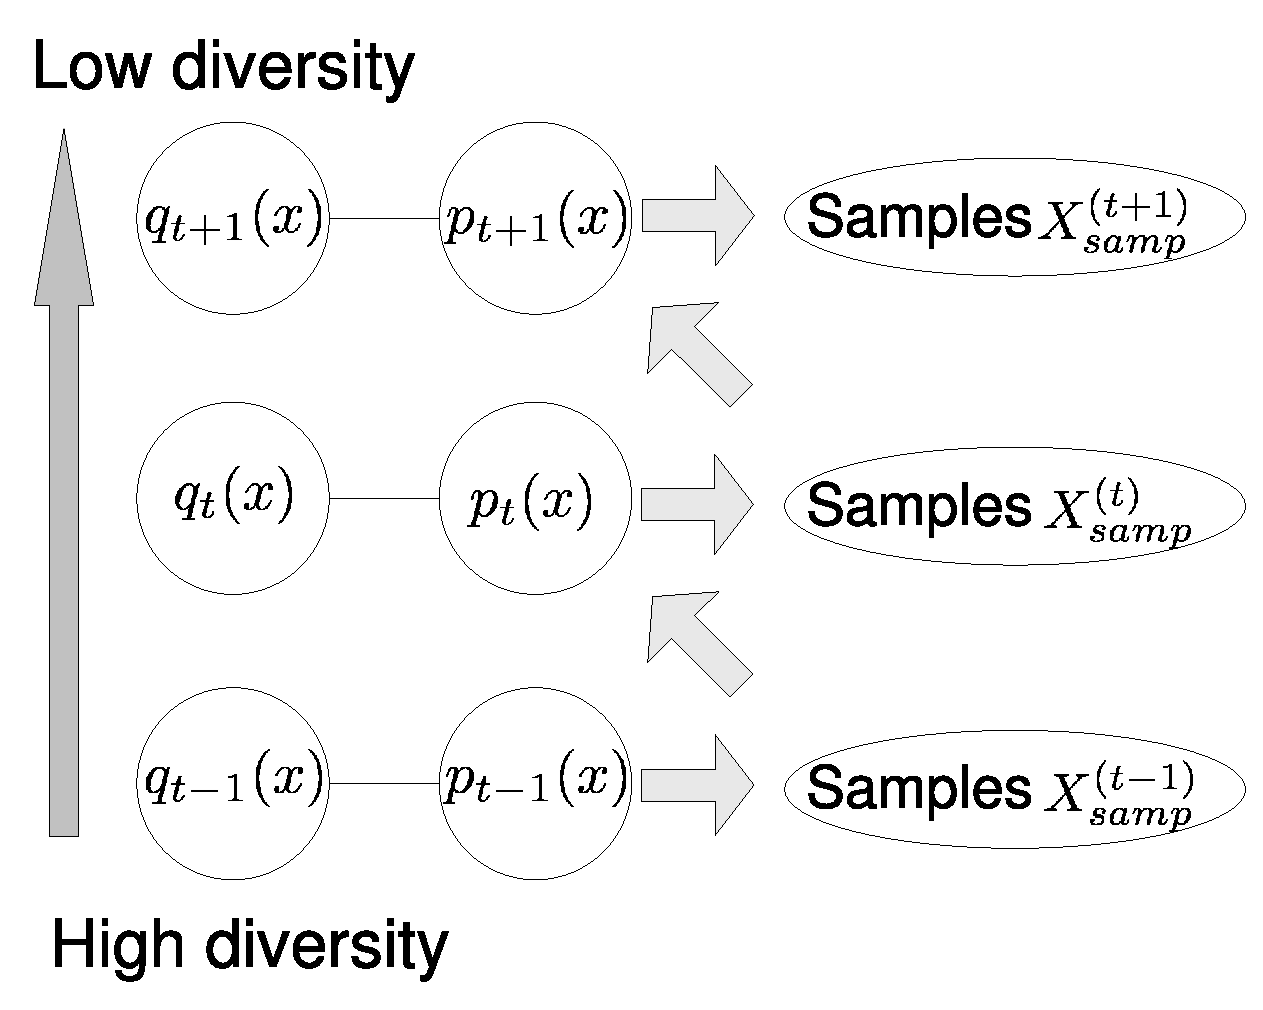
\includegraphics[width=\hfiglength\linewidth]{data_etc/annealing.eps}}
\caption{Illustration of Annealing.}
\label{fig_annealing}
\end{center}
\end{figure}


\section{A  Practical Approximation}
Although the EAPM seems to work well theoretically,
not in practice. 
%%experiment
The reason can be that
the variation of $\frac{q(x)}{p_{t-1}(x)}$ in (\ref{eapm-ml})
becomes too big.
To overcome this problem,
a slightly different method is often employed in practice.
This algorithm is called the estimation of distribution algorithm (EDA) in
this thesis. 

The difference from the EAPM is that
EDA does not use importance sampling.
Instead of (\ref{eapm-ml}), 
EDA performs
\begin{equation}
  p_{t}(x)=\argmax_{\hat p_{t}(x)} \frac{1}{M} \sum I(f(x)<\tilde f_t)\log
  \hat p_{t}(x).
\label{eda-ml}
\end{equation}
This means that promising solutions are selected from the
generated samples according to their cost function value
and
then the distribution of the selected solutions are estimated.
This selection manner is called the truncation selection.
(\ref{eda-ml}) can be easily derived from (\ref{eapm-ml}) by
supposing that $p_{t-1}(x)=q_{t-1}(x)$,
each $q_{t}(x)$ is a partially uniform distribution, and $f_{t-1}<f_t$.
This implies that EDA assumes that $p_{t-1}(x)$ 
completely approximate $q_{t-1}(x)$.
The pseudo-code is shown in Fig. \ref{eda-style-algo}.
Experimental comparisons between the EAPM and EDA are 
shown in Appendix \ref{exp-edace}.
The experiments show that EDA outperforms the EAPM.
However,
this thesis do not recommend\footnote{
This thesis recommends another form of (\ref{eapm-ml}) as follows:
\begin{equation}
 p_{t}(x)=\argmax_{\hat p_{t}(x)} \frac{1}{N} \sum 
\left(
\frac{q_t(x)}{p_{t-1}(x)}
\right)^r
\log \hat p_{t}(x),
\label{aeapm-ml}
\end{equation}
where $0 \leq r \leq 1$.
This form is friendly to importance sampling and
we can represent the EDA by $r=0$.
}
 this type of approximation
and the proposed methods in the following sections are
extensions of the EAPM.


\begin{figure}[tbp]
\renewcommand{\arraystretch}{1.23}
\centering
\begin{tabular}{lp{.9\linewidth}}
\multicolumn{2}{c}{Estimation of Distribution Algorithm (EDA)}\\
\hline
1 & Initialization: Generate samples $X^{(0)}_{samp}=\{x_i\}_1^M $ from the uniform
 distribution $p_0(x)$. $t \Leftarrow 1$.\\
2 & do\{ \\
3 & \algoindent Determine the threshold parameter $f_t$. \\
4 & \algoindent \parbox[t]{\algoremain}{Calculate the empirical log-likelihood according to (\ref{eda-ml}) from $X^{(t-1)}_{samp}$.}\\
5 & \algoindent Build a probability model $p_t(x)$ of $X^{(t)}_{pop}$.\\
6 & \algoindent Generate samples $X^{(t)}_{samp}=\{x_i\}_1^M $ from $p_t(x)$.\\
7 & \algoindent $t \Leftarrow t+1$.\\
8 & \}until(stopping criterion reached)\\
\hline
\end{tabular}
%\vspace{3mm}
\caption{The Pseudo-code of EDA.}
\label{eda-style-algo}
\end{figure}






